\documentclass[12pt,a4paper,twoside,openright,titlepage,final]{article}
\usepackage{fontspec}
\usepackage{amsmath}
\usepackage{amsfonts}
\usepackage{amssymb}
\usepackage{makeidx}
\usepackage{graphicx}
\usepackage[hidelinks,unicode=true]{hyperref}
\usepackage[spanish,es-nodecimaldot,es-lcroman,es-tabla,es-noshorthands]{babel}
\usepackage[left=3cm,right=2cm, bottom=4cm]{geometry}
\usepackage{natbib}
\usepackage{microtype}
\usepackage{ifdraft}
\usepackage{verbatim}
\usepackage[nottoc]{tocbibind}
\usepackage{pdflscape}
\usepackage[obeyDraft]{todonotes}
\ifdraft{
	\usepackage{draftwatermark}
	\SetWatermarkText{BORRADOR}
	\SetWatermarkScale{0.7}
	\SetWatermarkColor{red}
}{}
\usepackage{booktabs}
\usepackage{longtable}
\usepackage{calc}
\usepackage{array}
\usepackage{caption}
\usepackage{subfigure}
\usepackage{footnote}
\usepackage{url}
\usepackage[titletoc]{appendix}

\setsansfont[Ligatures=TeX]{texgyreadventor}
\setmainfont[Ligatures=TeX]{texgyrepagella}
\setmonofont{FreeMono}

\usetikzlibrary{decorations.pathreplacing}

%*******************************************************
%                 NO MODIFICAR
\newcommand*{\FSfont}[1]{%
  \fontencoding{T1}\fontfamily{#1}\selectfont}

\newlength{\tpheight}\setlength{\tpheight}{0.9\textheight}
\newlength{\txtheight}\setlength{\txtheight}{0.9\tpheight}
\newlength{\tpwidth}\setlength{\tpwidth}{0.9\textwidth}
\newlength{\txtwidth}\setlength{\txtwidth}{0.9\tpwidth}
\newlength{\drop}
%*******************************************************

% Crea una portada con los siguientes parámetros
%
% #1 : Título 
% #2 : Subtítulo
% #3 : Subsubtítulo
% #4 : Autor(es)
% #5 : Lugar
%

\newcommand*{\portada}[5]{
\begin{titlepage}
\begingroup
\vspace*{1cm}
\drop = 0.2\txtheight
\centering
\vfill
{\Huge \scshape #1}\\[\baselineskip]
{\Large \textbf{#2}}\\[\baselineskip]
{\Large \scshape #3}\\[\baselineskip]
\vspace*{0.3cm}
{\large \textit{#4}}\\[0.5\drop]

\includegraphics[scale=0.35]{./imagenes/logoURJC.jpg}
\vspace*{1.5cm}

{\large \scshape #5, \today} \par
\begin{center}
\end{center}
\vfill\null
\endgroup
\end{titlepage}
}
 %*****************************************************
 


\author{José Ignacio Escribano}

\title{}

\setlength{\parindent}{0pt}
\usepackage{fancyvrb}

\begin{document}

\pagenumbering{alph}
\setcounter{page}{1}

\portada{Caso Práctico I}{Minería de datos}{Componentes principales y análisis de correspondencias}{José Ignacio Escribano}{Móstoles}

\listoffigures
\thispagestyle{empty}
\newpage

\listoftables
\thispagestyle{empty}
\newpage

\tableofcontents
\thispagestyle{empty}
\newpage


\pagenumbering{arabic}
\setcounter{page}{1}

\section{Introducción}

En este caso práctico, utilzaremos distintas bases de datos para poner en práctica lo aprendido sobre componentes principales y análisis de correspondencias.\\

En la primera cuestión de evaluación relizaremos un análisis de componentes principales y en la segunda un análisis de correspondecias. En ambos casos utilizaremos el software estadístico R.

\section{Resolución de las cuestiones de evaluación}

\subsection{Primera cuestión}

En esta primera cuestión, debemos realizar un análisis de componentes principales con los datos gabriel1971 del paquete bpca de R. En él se recogen las comodidades de hogares en varias zonas de Jerusalén.\\

Para comenzar con el PCA, observamos las variables y los datos (por su pequeño tamaño) de los que consta esta base de datos:

\begin{Verbatim}[fontsize=\scriptsize]
             CRISTIAN ARMENIAN JEWISH MOSLEM MODERN.1 MODERN.2 OTHER.1 OTHER.2  RUR
toilet           98.2     97.2   97.3   96.9     97.6     94.4    90.2    94.0 70.5
kitchen          78.8     81.0   65.6   73.3     91.4     88.7    82.2    84.2 55.1
bath             14.4     17.6    6.0    9.6     56.2     69.5    31.8    19.5 10.7
eletricity       86.2     82.1   54.5   74.7     87.2     80.4    68.6    65.5 26.1
water            32.9     30.3   21.1   26.9     80.1     74.3    46.3    36.2  9.8
radio            73.0     70.4   53.0   60.5     81.2     78.0    67.9    64.8 57.1
tv set            4.6      6.0    1.5    3.4     12.7     23.0     5.6     2.7  1.3
refrigerator     29.2     26.3    5.3   10.5     52.8     49.7    21.7     9.5  1.2
\end{Verbatim}

Tenemos 8 variables en esta base de datos: CRISTIAN (cristianos), ARMENIAN (armenios), JEWISH (judíos), MOSLEM (musulmanes), MODERN.1 (modernos.1), MODERN.2 (modernos.2), OTHER.1 (otros.1), OTHER.2 (otros.2) y RUR (población rural).\\

Las comodidades de los hogares son lavabo, cocina, baño, electricidad, agua, radio, televisión y nevera.\\

Antes de realizar el PCA, realizamos un resumen de cada variable para ver si existen grandes diferencias de escala entre las variables.

\begin{Verbatim}[fontsize=\scriptsize]
   CRISTIAN        ARMENIAN         JEWISH           MOSLEM         MODERN.1       
 Min.   : 4.60   Min.   : 6.00   Min.   : 1.500   Min.   : 3.40   Min.   :12.70  
 1st Qu.:25.50   1st Qu.:24.12   1st Qu.: 5.825   1st Qu.:10.28   1st Qu.:55.35   
 Median :52.95   Median :50.35   Median :37.050   Median :43.70   Median :80.65   
 Mean   :52.16   Mean   :51.36   Mean   :38.038   Mean   :44.48   Mean   :69.90   
 3rd Qu.:80.65   3rd Qu.:81.28   3rd Qu.:57.275   3rd Qu.:73.65   3rd Qu.:88.25   
 Max.   :98.20   Max.   :97.20   Max.   :97.300   Max.   :96.90   Max.   :97.60  
 
    MODERN.2        OTHER.1         OTHER.2           RUR        
 Min.   :23.00   Min.   : 5.60   Min.   : 2.70   Min.   : 1.200  
 1st Qu.:64.55   1st Qu.:29.27   1st Qu.:17.00   1st Qu.: 7.675  
 Median :76.15   Median :57.10   Median :50.50   Median :18.400  
 Mean   :69.75   Mean   :51.79   Mean   :47.05   Mean   :28.975  
 3rd Qu.:82.47   3rd Qu.:72.00   3rd Qu.:70.17   3rd Qu.:55.600  
 Max.   :94.40   Max.   :90.20   Max.   :94.00   Max.   :70.500  
\end{Verbatim}

Puesto que todas las variables son porcentajes, no será necesario escalar las variables.\\

Calculamos los autovalores de la matriz de covarianzas de cada componente principal. Tenemos lo siguiente:

\begin{Verbatim}[fontsize=\scriptsize]
Standard deviations:
[1] 9.320779e+01 1.832205e+01 1.270250e+01 6.285602e+00 4.360009e+00 3.173772e+00 1.334664e+00 4.637537e-15

Rotation:
                PC1          PC2         PC3         PC4         PC5         PC6        PC7         PC8
CRISTIAN -0.3774826  0.121218290  0.48084436  0.40488521  0.09488569  0.04718208  0.1684884  0.61020121
ARMENIAN -0.3705463  0.139480696  0.33349190  0.29316420 -0.12562056 -0.26551516 -0.5595880 -0.47868586
JEWISH   -0.3661639  0.283772155 -0.14629893 -0.48523653  0.63125444  0.05070960 -0.3147304  0.15768194
MOSLEM   -0.3830485  0.206214896  0.21868882 -0.33508268 -0.07215394 -0.15428314  0.6858741 -0.38841777
MODERN.1 -0.2712244 -0.650316615  0.08542964  0.11706375  0.31135408  0.53403172  0.0548636 -0.30654238
MODERN.2 -0.2201737 -0.555023062 -0.20049950 -0.05554059  0.08031210 -0.72925238  0.0137473  0.14695975
OTHER.1  -0.3214890 -0.189304742 -0.14718330 -0.06899714 -0.33431892  0.08981627  0.0167303  0.28706773
OTHER.2  -0.3710368  0.007994056 -0.20526225 -0.28162871 -0.58680361  0.27449421 -0.2179725  0.08803244
RUR      -0.2762924  0.275567693 -0.69068799  0.54911184  0.10967589  0.02208732  0.1949449 -0.13061157
\end{Verbatim}

Tenemos que las dos primeras componentes principales acumulan más del 95\% de la varianza de los datos.\\

Podemos ver estos datos de forma más gráfica en la Figura~\ref{fig:varianza_pca}.\\

\begin{figure}[tbph!]
\centering
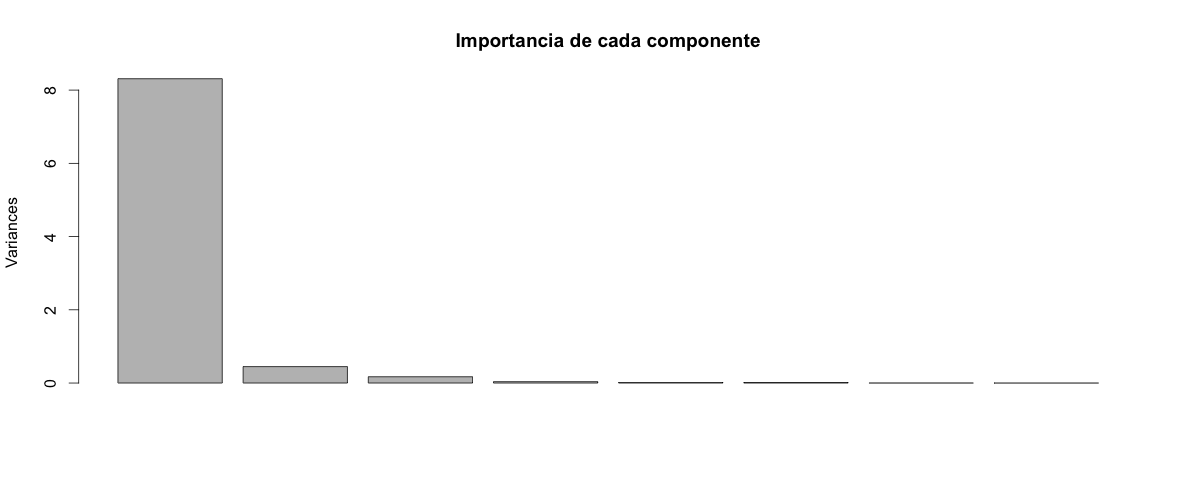
\includegraphics[width=0.8\linewidth]{imagenes/varianza_pca}
\caption{Importancia de cada componente}
\label{fig:varianza_pca}
\end{figure}

Existe una gran diferencia entre la primera y las otras componentes. De forma numérica se obtiene lo siguiente:

\begin{Verbatim}[fontsize=\scriptsize]
Importance of components:
                           PC1      PC2      PC3     PC4     PC5     PC6     PC7       PC8
Standard deviation     93.2078 18.32205 12.70250 6.28560 4.36001 3.17377 1.33466 4.638e-15
Proportion of Variance  0.9387  0.03627  0.01743 0.00427 0.00205 0.00109 0.00019 0.000e+00
Cumulative Proportion   0.9387  0.97496  0.99240 0.99667 0.99872 0.99981 1.00000 1.000e+00
\end{Verbatim}

La primera componentes explica más del 93\% de la varianza de los datos, y entre las dos primeras casi el 97.5\% de la varianza.\\

Cogeremos las dos primeras componentes para representar los datos en un diagrama de dispersión (Figura~\ref{fig:dos_componentes}).\\

\begin{figure}[tbph!]
\centering
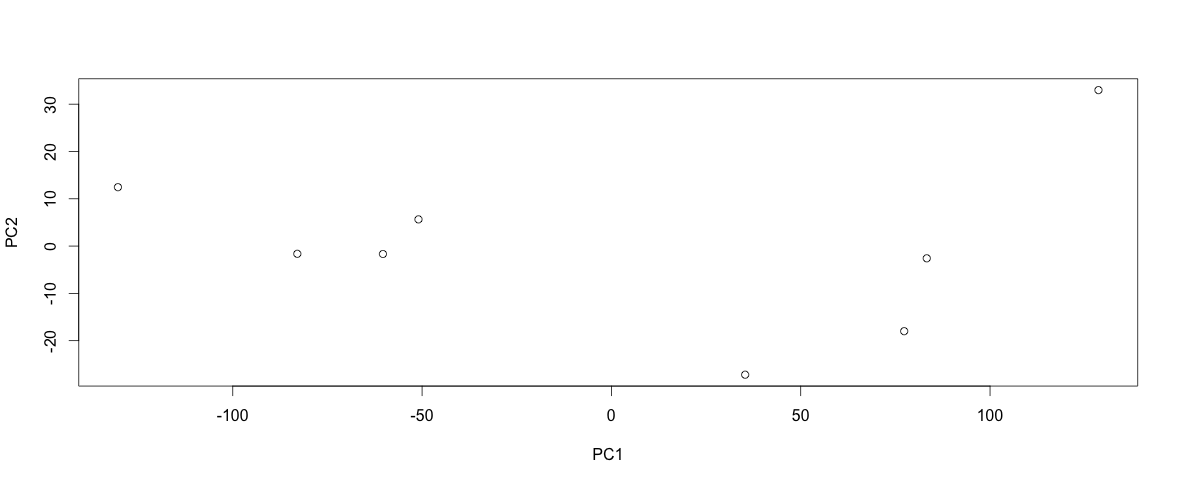
\includegraphics[width=0.8\linewidth]{imagenes/dos_componentes}
\caption{Proyección sobre las dos componentes principales}
\label{fig:dos_componentes}
\end{figure}

Este gráfico tiene difícil interpretabilidad, por lo que eliminamos los puntos y ponemos el nombre de cada comodidad (televisión, electricidad, baño, etc) como se puede ver en la Figura~\ref{fig:dos_componentes_nombres}.\\

\begin{figure}[tbph!]
\centering
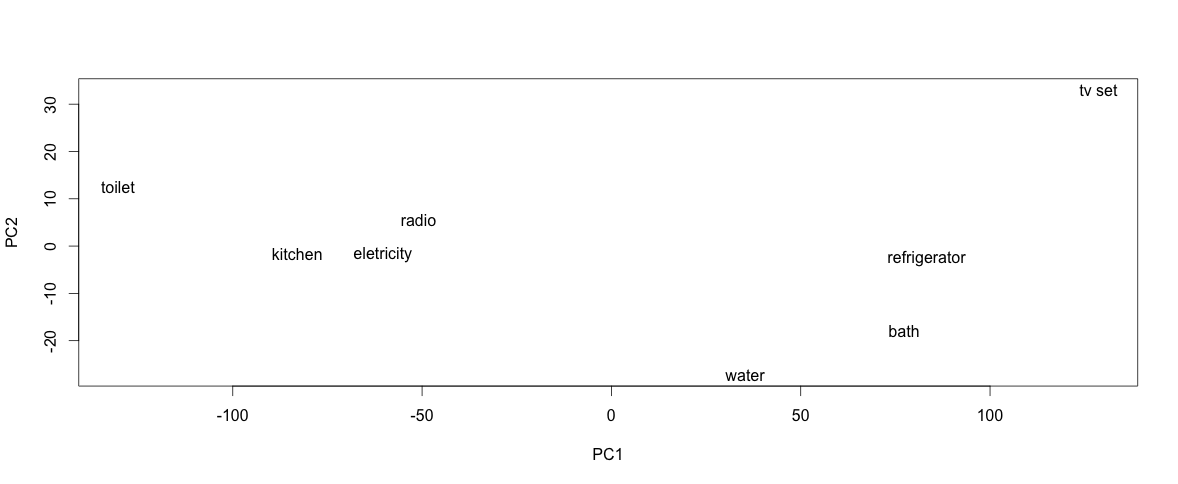
\includegraphics[width=0.8\linewidth]{imagenes/dos_componentes_nombres}
\caption{Proyección sobre las dos componentes principales con el nombre de las comodidades}
\label{fig:dos_componentes_nombres}
\end{figure}

Podemos mejorar el gráfico utilizando el biplot como se puede ver en la Figura~\ref{fig:biplot}\\

\begin{figure}[tbph!]
\centering
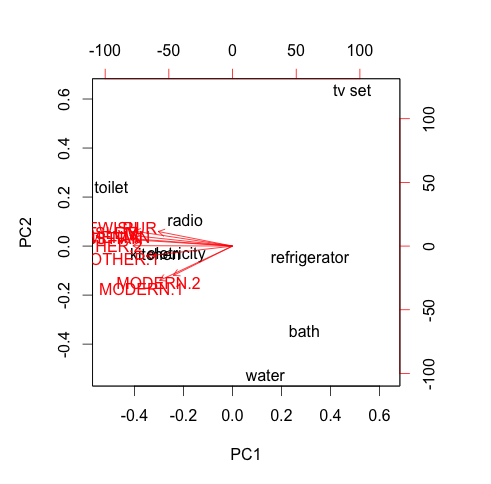
\includegraphics[width=0.5\linewidth]{imagenes/biplot}
\caption{Biplot}
\label{fig:biplot}
\end{figure}

\subsection{Segunda cuestión}



\section{Conclusiones}

\section{Código R}

\end{document}